\documentclass{beamer}
\usepackage[utf8]{inputenc}
\usepackage{tikz}
\usetikzlibrary{positioning}

\usepackage{utopia} %font utopia imported

\usetheme{Madrid}
\usecolortheme{default}

%------------------------------------------------------------
%This block of code defines the information to appear in the
%Title page
\title[Simulating the ground truth] %optional
{Simulating the ground truth}

\subtitle{Practical Course: Hands-on Deep Learning for Computer Vision and Biomedicine}

\author[Tim Kerschbaumer] % (optional)
{Tim Kerschbaumer}

\institute[] % (optional)
{
  \inst{1}%
  Department of Informatics\\
  Technichal University of Munich
}

\date[2017-08-28] % (optional)
{2017-08-28}

%End of title page configuration block
%------------------------------------------------------------



%------------------------------------------------------------
%The next block of commands puts the table of contents at the 
%beginning of each section and highlights the current section:

\AtBeginSection[]
{
  \begin{frame}
    \frametitle{Table of Contents}
    \tableofcontents[currentsection]
  \end{frame}
}
%------------------------------------------------------------


\begin{document}

%The next statement creates the title page.
\frame{\titlepage}


%---------------------------------------------------------
%This block of code is for the table of contents after
%the title page
\begin{frame}
\frametitle{Table of Contents}
\tableofcontents
\end{frame}
%---------------------------------------------------------


\section{Introduction}

\begin{frame}
\frametitle{Motivation}
\begin{itemize}
\item<1-> Supervised learning requires ground truth output targets for training and validation
\item<2-> In many applications the ground truth cannot be directly obtained
\item<3-> One field where data and labels are expensive to obtain is in diffusion MRI
\item<4-> Is it good enough to build and train models from computer simulations of the ground truth?
\end{itemize}
\end{frame}

\begin{frame}
\frametitle{Diffusion MRI}
\begin{itemize}
\item<1->Diffusion is the microscopic movement of atoms and molecules in a solution or gas.
\item<2->Molecules such as water floats freely through our bodies
\item<3->In some medical conditions, such as stroke, these molecules can become restricted.
\item<4->With diffusion MRI we measure the ability of these molecules to move freely within each voxel.
\end{itemize}
\end{frame}

\begin{frame}
\frametitle{Diffusion MRI}
\begin{figure}[h]
    \centering
    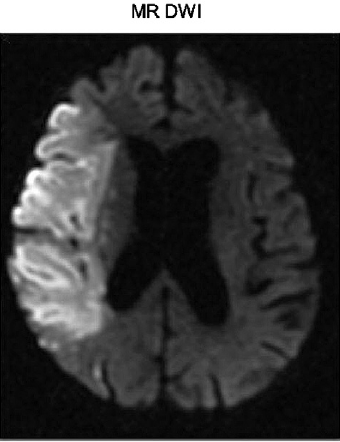
\includegraphics[scale=0.4]{stroke.png}
    \label{fig:mesh1}
    \caption{White area shows restricted diffusion}
\end{figure}
\end{frame}

\section{Methods}

\begin{frame}
\frametitle{Generating data}
How to generate data?
\begin{itemize}
\item<2->Camino Toolkit - Software tool for Diffusion MRI processing and simulation
\item<3->Input: Simulation configuration, i.e cylinder radius, the restricting environment where diffusion takes place.
\item<4->Output: A list of individual voxels with 288 channels (DWI signal intensity)
\end{itemize}

\pause
\pause
\pause
\pause

\begin{figure}[h]
    \centering
    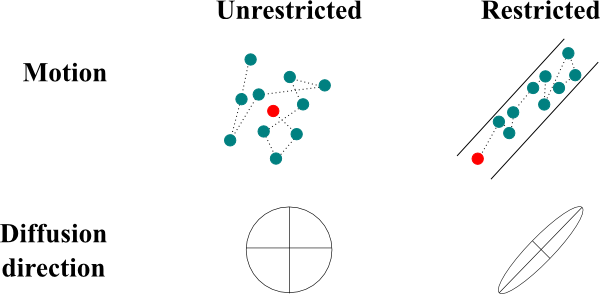
\includegraphics[scale=0.4]{brownianMotion.png}
    \label{fig:mesh1}
\end{figure}

\end{frame}

\begin{frame}
\frametitle{Generating data}
What data to generate?
\begin{itemize}
\item<2->Want similar to HPC (Human Connectome Project) - Diffusion MRI dataset from scanned persons
\item<3->Idea: Try wide spread of settings with Camino, use kNN to compare with HPC data.
\item<4->Run many simulations with these settings.
\end{itemize}
\end{frame}

\begin{frame}
\frametitle{Data}
\begin{itemize}
\item<1-> Each input is a voxel with 288-channels, i.e a $1 \times 1 \times 1 \times 288$ dimensional array.
\item<2-> Can simply be seen as a 288-dimensional feature vector, ignoring spatial $1 \times 1 \times 1$ dimensions.
\item<3-> Output is single value, cylinder radius, the input to each simulation.
\item<4-> Simulating data with Camino very slow, around 24 hours for 1000 voxels (with same setting) $\implies$ only have $93 900$ voxels.
\item<5-> Simulated data divided into training $60\%$, validation $20\%$ and test $20\%$.
\end{itemize}

\end{frame}

\begin{frame}
Network considerations
\frametitle{Developing the network}
\begin{itemize}
\item<2-> Different feed-forward architectures
\item<3-> L1 or L2 loss function
\item<4-> Which optimizer and what learning rate
\item<5-> Dropout and regularization
\item<6-> Standardization, scaling and batch normalization
\end{itemize}
\end{frame}

\begin{frame}
\frametitle{Evaluation}
Metrics for evaluating regression model performance \\
\pause
For $n$ samples:
\begin{itemize}
\item<2->Mean squared error between prediction $y$ and target $t$ as $\frac{1}{n} \sum_{i=1}^n (y_i-t_i)^2$
\item<3->$R^2$-score, $1 - \frac{SS_{res}}{SS_{tot}}$ where $SS_{res} = \sum_{i=1}^n(y_i - t_i)^2$ and $SS_{tot} = \sum_{i=1}^n(t_i - \overline{t})^2$. \\ Best possible score $1.0$.
\end{itemize}
\end{frame}

\section{Results and Discussion}

\begin{frame}
\frametitle{Model comparison}
\begin{itemize}
\item<1->Bigger networks in either depth or width not increasing model performance
\item<2->Small dropout fraction improves validation score, no further regularization needed
\item<3->L2 loss works better, expected since we simulate data and should not have many outliers
\item<4->Batch normalization does not improve, expected since data is already normalized and network not too deep
\item<5->Scaling outputs to $[0,1]$ was essential to get any presentable score, since targets very small, around $10^{-7}$
\end{itemize}
\end{frame}

\begin{frame}
\frametitle{Model comparison}
\begin{columns}

\column{0.5\textwidth}
\begin{figure}[h]
    \centering
    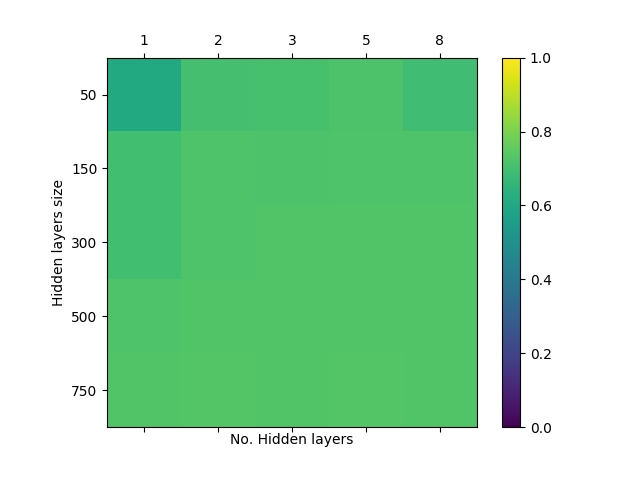
\includegraphics[scale=0.4]{heat-plot-depth-vs-width.png}
    \label{fig:mesh1}
    \caption{Heat plot showing $R^2$-score for hidden layer size vs depth}
\end{figure}

\column{0.5\textwidth}
\begin{figure}[h]
    \centering
    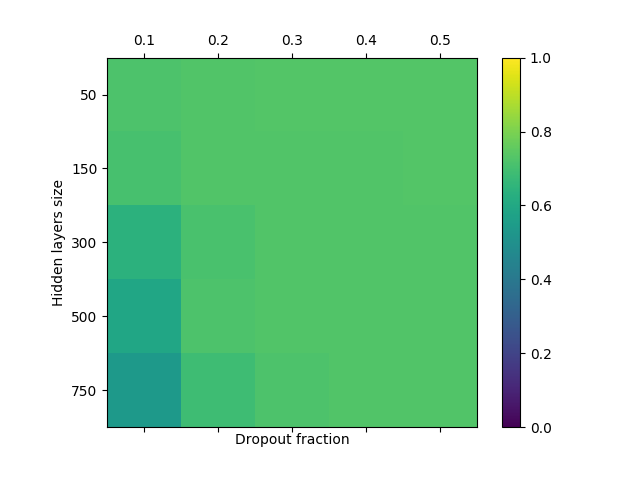
\includegraphics[scale=0.4]{heat-plot-dropout-vs-width.png}
    \label{fig:mesh2}
    \caption{Heat plot showing $R^2$-score for hidden layer size vs dropout fraction}
\end{figure}

\end{columns}
\end{frame}

\begin{frame}
\frametitle{Network}
Best network configuration
\begin{itemize}
\item<1-> Simple feedforward network with 3 hidden layers
\item<2-> ReLU activation functions in all but last layer (linear)
\item<3-> L2 loss function
\item<4-> Scaled outputs between $[0,1]$ since targets very small, around $10^{-7}$
\item<5-> Adam optimizer with learning rate $2.5*10^{-4}$
\end{itemize}

\pause
\pause
\pause
\pause
\pause

Test set performance:
\begin{itemize}
\item $R^2 = 0.80701$
\item $MSE = 1.77545 \times 10^{-14}$
\end{itemize}
\end{frame}

\begin{frame}
\frametitle{Network}
\begin{columns}

\column{0.5\textwidth}
\begin{figure}[h]
    \centering
    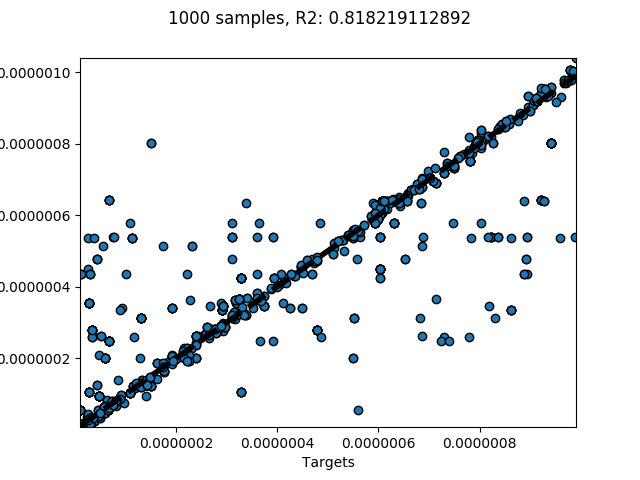
\includegraphics[scale=0.4]{diff-plot.png}
    \label{fig:mesh1}
    \caption{Predictions vs Targets on 1000 unseen random samples on best performing model}
\end{figure}

\column{0.5\textwidth}
\begin{figure}[h]
    \centering
    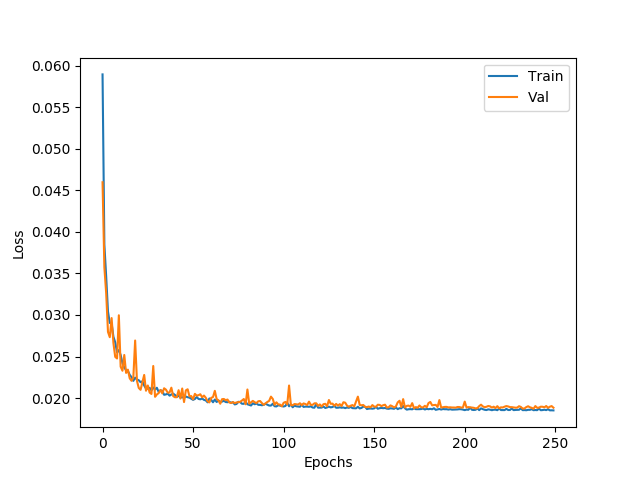
\includegraphics[scale=0.4]{loss-plot.png}
    \label{fig:mesh2}
    \caption{Loss vs Epochs on best performing model}
\end{figure}

\end{columns}

\end{frame}

\section{Conclusions}
\begin{frame}
\frametitle{Conclusions}
\begin{itemize}
\item<1->Camino Toolkit at its current state requires a large number of processors to generate big data in reasonable time.
\item<2->Having a regression model with multiple outputs would increase the expressiveness and complexity of the model
\item<3->Using more complex simulations, i.e not cylinders, would probably be closer to actual diffusion MRI data
\item<4->Training and test error very similar even without regularization, may indicate very similar inputs.
\item<5->Very easy to learn an "OK” network, very hard to improve on those results.
\item<6->Difficulty to get high train accuracy may indicate that the problem is ill-posed, i.e inputs are not uniquely mappable to targets.
\end{itemize}
\end{frame}

\begin{frame}
\begin{center}
\Huge Thank you for your attention\\
\Huge Questions?
\end{center}
\end{frame}

\end{document}